\section{Background Considerations}\label{sec:backgrounds} 

In order to support the broad physics reach of a next-generation experiment, multiple background sources must be considered. In addition to improved xenon purification, further scrutiny of materials in assays and exploration of discrimination techniques will be necessary to minimize backgrounds for rare event searches. The choice of host facility and detector design are also important considerations that will impact which and how backgrounds manifest. Modelling of detector performance and simulations of background events will be critical in informing the design of the experiment, deriving sensitivities, and ultimately in achieving final science results~\cite{Undagoitia:2015gya}.

\subsection{Underground Laboratories}

Muons traversing detectors or surrounding materials will induce primary backgrounds as well as secondary neutrons and cosmogenic backgrounds from activation of materials~\cite{Mei:2005gm,Kudryavtsev:2008fi}. Dark matter detectors are thus deployed in deep underground laboratories, where cosmic-ray muon backgrounds are greatly reduced by the rock overburden~\cite{Bettini:2014tva}. Nevertheless, for high-sensitivity experiments, active muon shielding is still required in order to tag remaining muon-related background events and reduce the muon-induced background to a negligible level compared to other sources. Muon fluxes at the typical underground laboratories range from 1~muon/m$^2$/hour at the Laboratori Nationali del Gran Sasso  (LNGS, 3,100 meters water equivalent deep)~\cite{Mei:2005gm,Votano:2012fr} to about 5~muons/m$^2$/month at China's Jinping underground laboratory (CJPL, 6,720 meters water equivalent deep)~\cite{Yu-Cheng:2013iaa, Cheng:2018lcf} (\autoref{fig:muonflux}).

\begin{figure}[!htbp]
\begin{center}
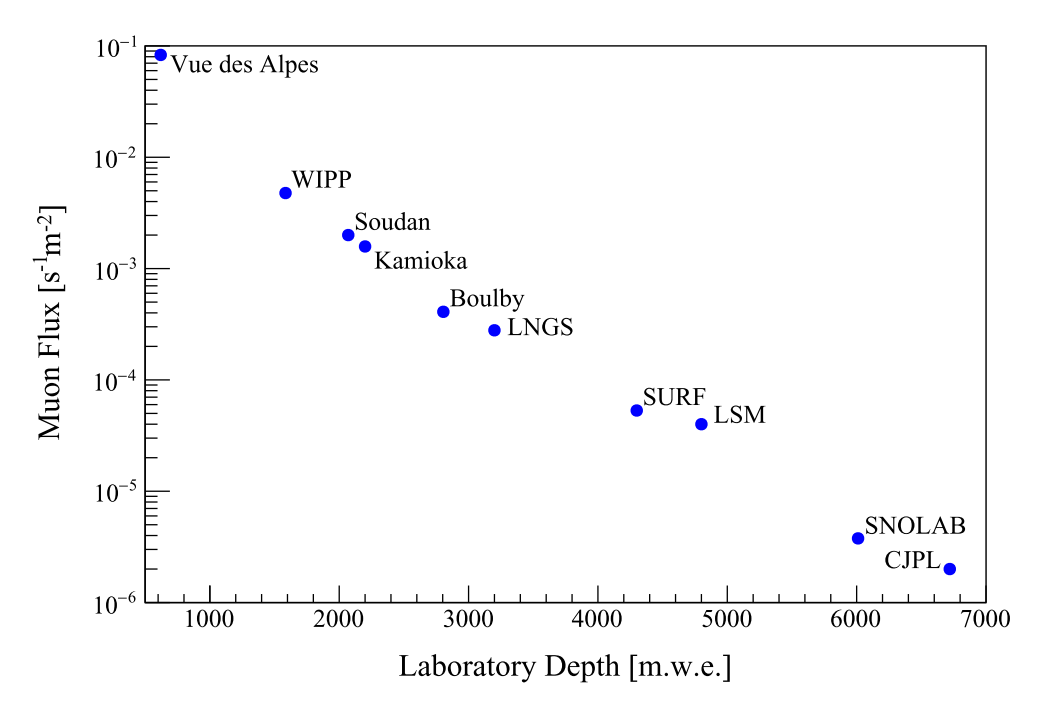
\includegraphics[width=0.99\columnwidth]{fig_muon_flux.png}
\caption{Depth-dependent muon flux at various underground laboratories (measured in “meters water equivalent” (m~w.e.). While the depth increases from 620 m.w.e. to 6720 m.w.e, the muon flux decreases by more than four orders of magnitude. Figure from~\cite{Schumann:2019eaa}.}\label{fig:muonflux}
\end{center}
\end{figure}
  
There are a host of underground laboratories that can be considered as location for the next-generation observatory discussed here. This includes the laboratories hosting the current generation of liquid xenon detectors: LNGS~\cite{Bettini:2007xc} (location of XENONnT), CJPL~\cite{Li:2014rca} (location of PandaX-4T) and SURF~\cite{Heise:2017rpu} (location of LZ). The Boulby Underground Laboratory has a similar muon flux to LNGS with notably low radon levels~\cite{Paling:2015ss}, and a world-class background screening facility~\cite{Scovell:2018ap}. The Modane Underground Laboratory~\cite{Piquemal:2012fs} includes a facility for radon-free air, and the entire scientific campus of SNOLAB~\cite{Lawson:2012sga} is equipped as a cleanroom with some of the lowest available muon flux. Several of these laboratories entertain feasibility studies for creating additional underground space for scientific use. All in all, there is a favorable outlook that suitable underground space can be made available for the next-generation liquid xenon observatory.

\subsection{Fiducialization}\label{sec:erfiducialization}

The dominant background component in liquid xenon detectors at a given energy range has evolved with increasing detector size. In earlier detectors (e.g.~XENON100~\cite{Aprile:2011vb}, LUX and PandaX-I/II), the gamma radiation from radioactive contaminants of detector construction materials contributed significantly to the electronic recoil background for dark matter searches in the keV energy range. A fiducial volume selection is typically applied to reduce these backgrounds, which predominantly appear towards the boundaries of the bulk xenon: with larger detector masses and hence smaller surface-to-volume ratios, fiducialization can preserve a higher proportion of the active volume for a physics search. Gamma-induced electronic recoils will remain a significant background for rare event searches at the MeV scale such as the $0\nu \beta \beta$-decay of $^{136}$Xe (\autoref{sec:0nubb}, \autoref{fig:0vbb_signal}).

Radioactive contaminants of detector materials are also the source of radiogenic neutrons through spontaneous fission or $(\alpha,\mathrm{n})$ reactions. Fiducialization of the liquid xenon target is not quite as effective for neutrons compared to gamma radiation. Therefore, current and future liquid xenon detectors are equipped with dedicated neutron veto systems for efficient mitigation of nuclear recoil background events.

\subsection{Material Selection}

The selection of materials featuring the lowest contamination with radioactive impurities is the most important strategy for background mitigation in current and future liquid xenon experiments \cite{Aprile:2017ilq,Akerib:2020com}. Trace amounts of uranium and thorium can be detected by means of highly sensitive gamma-spectrometers, ICPMS measurements or neutron activation analysis. Radon emanation rates are determined in dedicated setups where the radon which is emanating from the sample accumulates in an ambient carrier gas, before the radon activity in this sample gas is measured, typically using proportional counters or electrostatic radon monitors~\cite{Akerib:2020com,Aprile:2020vmn}. 

Various material samples are measured in intensive screening campaigns in order to pre-select and built radiopure detector components which fit the requirements for a next-generation liquid xenon experiment~\cite{XENON:2015ara}. Once the materials are selected, the screening measurements are used for background modeling by means of simulation. Precise knowledge of emanation sources can further be used to optimize the online purification systems.

\subsection{Intrinsic Background Mitigation}

Sources of so-called intrinsic backgrounds are typically radioactive noble gases which are homogeneously mixed within the liquid xenon target. Thus, any type of shielding remains ineffective. Trace amounts of $^{85}$Kr that stay in the xenon during its distillation from air will cause, if not removed, a low-energy electronic recoil background from its beta decay. Due to the absence of krypton sources within the detector, the $^{85}$Kr contamination is constant over time and scales with the liquid xenon mass. $^{85}$Kr thus needs to be removed through cryogenic separation of the xenon target, as pioneered by the XMASS collaboration~\cite{Abe:2008py}. The purification of xenon from trace amounts of $^{85}$Kr has been successfully demonstrated using both cryogenic distillation~\cite{Abe:2008py,Wang:2014ehv,Aprile:2016xhi} and adsorption~\cite{Bolozdynya:1997,Akerib:2016hcd} as separation techniques. Cryogenic distillation in particular is appropriate to process large amount of xenon gas before being filled into the experiment, but also an online krypton purification at a running detector has been demonstrated. Starting with a $^{85}$Kr contamination of several ppm in commercial xenon, a purification down to 8\,ppq $^{85}$Kr in xenon has been achieved by means of cryogenic distillation~\cite{Lindemann:2013kna}. This level is well below even the requirements of a next-generation liquid xenon experiment.

$^{222}$Rn is not immanent in the xenon gas, but continuously emanates from surfaces of detector materials. Due to its subsequent beta decays, radon is the dominant background source in current liquid xenon detectors. A smaller surface-to-volume ratio will naturally decrease the radon concentration in next-generation liquid xenon detectors. However, further mitigation strategies are needed to achieve a level of about $0.1\1{\mu Bq/kg}$ that is required in order to render radon-induced backgrounds sub-dominant versus the irreducible contributions from neutrino signals. Once a new detector has been built, its emanation rate of $^{222}$Rn is set and expected to be constant over the lifetime of the experiment. A further suppression of the radon induced background can be achieved through continuous purification of the xenon target. The key for an efficient radon removal is a good separation technique and a high purification flow which revolves the entire xenon target fast with respect to the 3.8\,d half-life of radon. Radon removal based on cryogenic distillation has been successfully tested in large scale liquid xenon experiments~\cite{Aprile:2017kop} and will be used also in XENONnT. Radon purification systems designed for small purification flows can also significantly reduce the radon concentration in xenon. Since the dominating radon emanation sources in an experiment are known from screening, dedicated purge flows towards the radon removal system can prevent radon to enter the liquid xenon target~\cite{Akerib:2020com}.

Another intrinsic background source is the decay of $^{137}$Xe. It is naturally created inside the xenon target through activation by muon-induced neutrons. Thus, the $^{137}$Xe induced background strongly depends on the muon rate at the experimental site.

\subsection{Isolated Light and Charge Signals and Accidental Coincidences} 

Due to the proportional amplification of charge in liquid xenon TPCs, even a single extracted electron can produce a detectable S2 of tens of photoelectrons in size~\cite{Burenkov:2009zz,Santos:2011ju,Angle:2011th,Aprile:2013blg,Edwards:2017emx,Xu:2019dqb}. A standalone search with S2s (i.e.~without requiring an accompanying S1 signal, see \autoref{sec:s2only} on page~\pageref{sec:s2only}) can thus lower the energy threshold, improving the reach to low-mass WIMPs, solar axions and solar neutrinos, and other physics that have associated low-energy recoil signatures~\cite{Aprile:2019xxb}. However, this sensitivity to any process that can knock out even single electrons from their shell brings in additional instrumental backgrounds. Several sources of S2-only, single and few-electron backgrounds are known and being further investigated~\cite{Akerib:2020jud, Kopec:2021ccm, Bodnia:2021flk, Akimov:2016rbs, Aprile:2013blg, Sorensen:2017kpl, Sorensen:2017ymt}. Photoionization backgrounds caused by large S2s die away within a maximum drift time after the S2~\cite{Aprile:2013blg}. Emission from metal surfaces would be evident in specific locations that could be avoided with positional cuts. The most impactful background appears to be S2s up to five electrons in size that continue for times up to seconds after a large S2. The rates of these correlated small S2s, which appear in the same location as a previous large S2, decrease according to a power law with time after the large S2~\cite{Kopec:2021ccm}. This background can be mitigated with positional and temporal cuts after large S2s.

\begin{figure}[!htbp]
\begin{center}
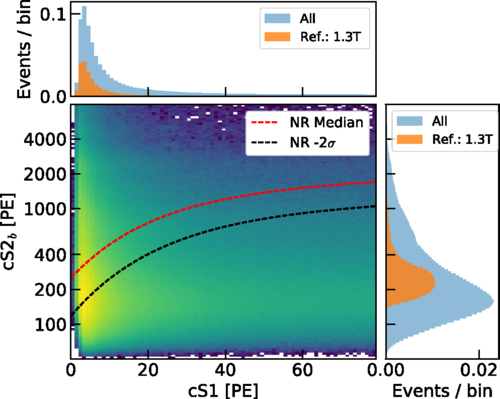
\includegraphics[width=0.95\columnwidth]{fig_x1t_accidentals.png}
\caption{Illustration of the accidental coincidence background distribution from XENON1T in cS1 and log10(cS2b), with projections on each axis showing the expected distribution within the entire analysis space (blue), and in the reference region for 1.3~tonne fiducial volume. The reference region lies between the nuclear recoil median and $-2\sigma$ quantile lines, marked by red and black lines, respectively. Figure from~\cite{Aprile:2019dme}.}\label{fig:accidental}
\end{center}
\end{figure}

S1-only backgrounds also exist due to interactions in areas insensitive to the charge channel, e.g.~outside of the main drift field region of the TPC (notably below the cathode), or other locations where there could be charge depletion or inability for elections to reach the extraction region, perhaps as a result of the field configuration towards the edges of the detector. Unrelated, isolated S1-only and S2-only signals can be close enough in time to be mis-identified as a single event. Such accidental coincidences of these instrumental backgrounds can thus mimic a physics interaction for a conventional search in S1-S2 phase space. As both lone S1s and S2s are more likely to manifest at smaller signal values, these accidental coincidence backgrounds are particularly problematic for the WIMP search region of interest. The absolute incidence of such accidental events should increase in a next-generation detector, as the corresponding surfaces and volumes from which lone S1s and S2s can arise become larger. However, a data-driven approach, as adopted for XENON1T (\autoref{fig:accidental}), should be sufficient to characterise this background. 

\subsection{Monte-Carlo Simulation of Backgrounds}

\subsubsection{Background Model} 

To construct a model of expected backgrounds, the activities and normalizations found from material assays and physics estimates must be paired with the corresponding detection efficiencies of the associated events. These efficiencies are determined through Monte Carlo simulations of event primaries, such as daughters from radioactive decay, within a realistic representation of the experiment. Simulations are used to determine the energy depositions from backgrounds within the detector, and in translating them into observed signals.

A framework based on the GEANT4 toolkit~\cite{Agostinelli:2002hh} allows for the tracking of particles within a rendering of the detector geometry. Custom additions can enhance the modelling of various physics processes and phenomena beyond the standard physics lists available, as in the case of modelling neutron captures on Gd using ANNRI~\cite{Hagiwara:2019ptep,Tanaka:2020ptep} or DICEBOX~\cite{Becvar:1998sd} derived outcomes for an improved veto assessment. Bespoke event generators enable the simulation and study of more involved scenarios that are not well-captured in default GEANT4, such as $(\alpha,\mathrm{n})$ reactions accompanied by a varying multiplicity of gammas, or events from atmospheric muons which penetrate the laboratory rock overburden~\cite{Akerib:2021ap}.

Analysis cuts can be applied to remove events with coincident scatters in veto detectors, and restrict to an energy region of interest and/or a fiducial volume. Persistent background counts can then be compared to those anticipated from potential signals. This approach has been used in predicting the background burden of many present-generation experiments, forming the basis of WIMP sensitivity estimates for XENONnT~\cite{Aprile:2020vtw}, LZ~\cite{Akerib:2018lyp} and PandaX-4T~\cite{Zhang:2018scp}. 

\subsubsection{Generation of S1 and S2 Signals}

\begin{figure*}[!htbp]
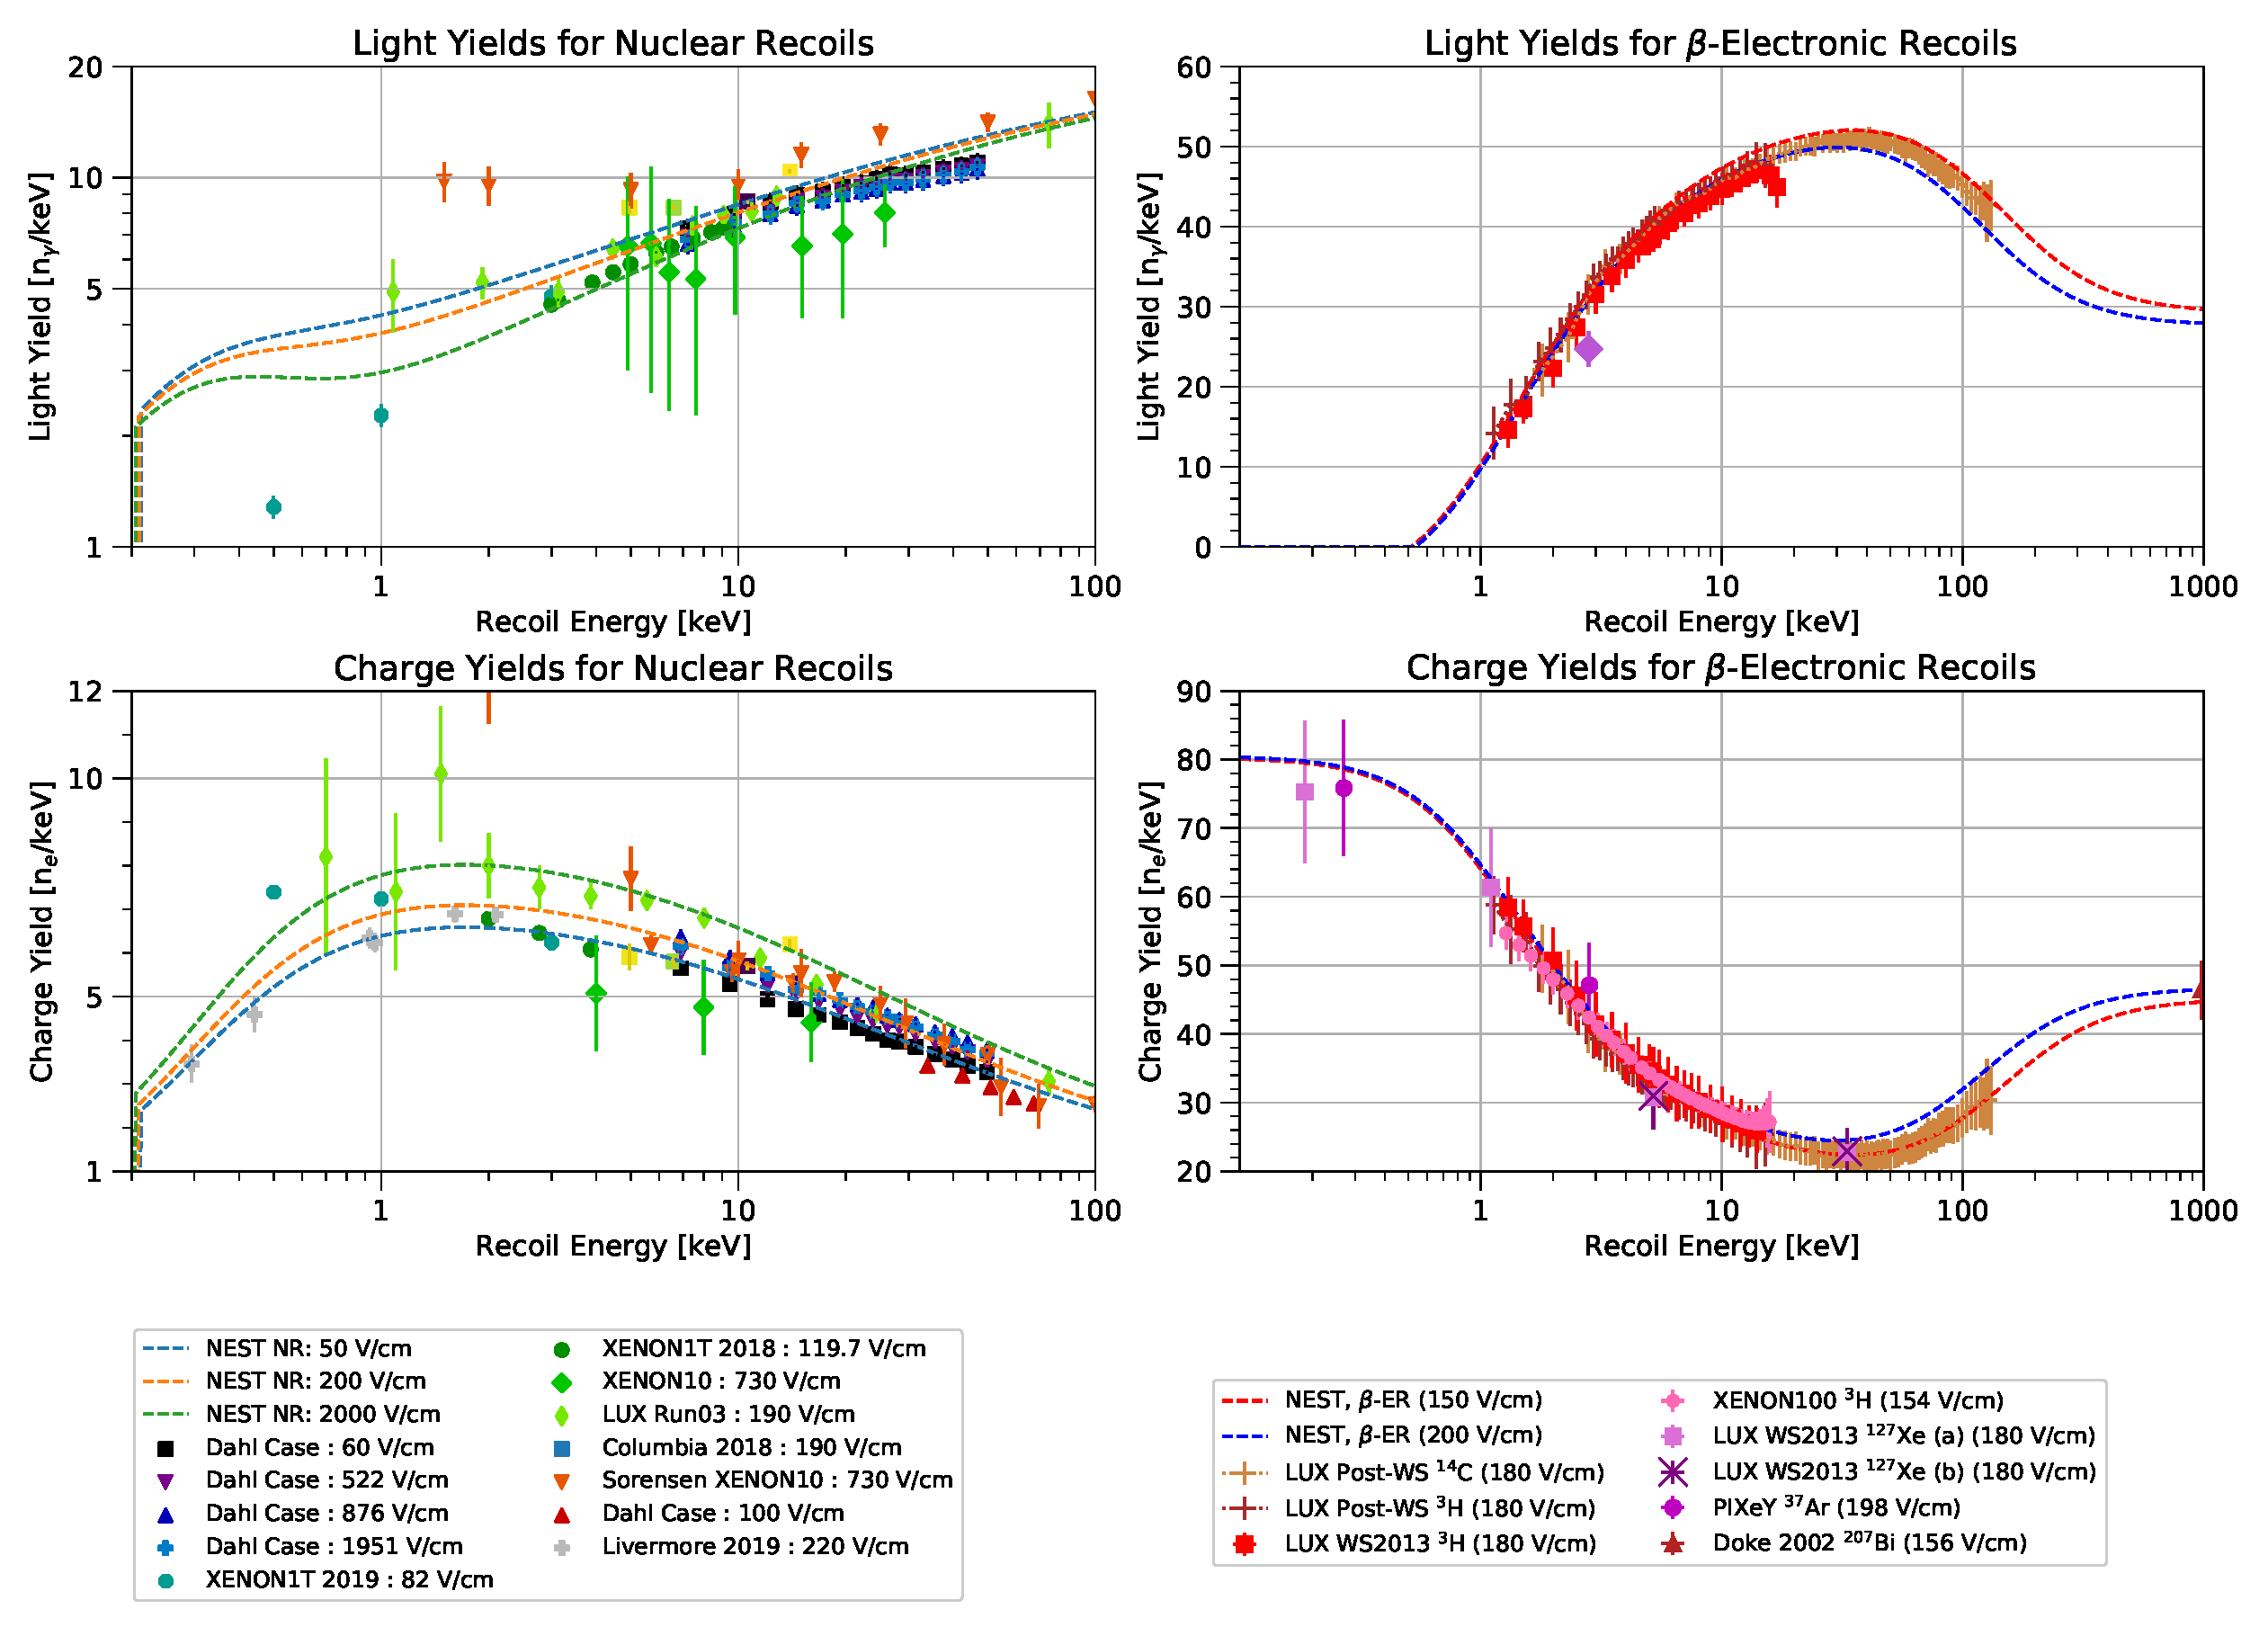
\includegraphics[width=2.05\columnwidth]{fig_nest_light_and_charge_yields.eps}
\caption{The light and charge yields for nuclear and electronic recoils, as measured by various experiments and as modeled by the Noble Element Simulation Technique (NEST)~\cite{szydagis_m_2020_3905382}. The light (charge) yield is defined as the number of photons (electrons) leaving the recoil site after electron-ion recombination, per unit energy. For electronic recoils, NEST has two models for $\beta$-induced and $\gamma$-induced recoils, respectively, and we show the $\beta$ model. Correspondingly, we only show experimental measurements from $\beta$ calibrations or low-energy line sources, which are observed to fit the $\beta$ model better than the $\gamma$ model.
The nuclear recoil data points are from E.~Dahl's thesis~\cite{Dahl:2009nta}, XENON1T~\cite{Aprile:2019dme, Lin:2018xenon1t}, XENON10~\cite{Sorensen:2008ec, Sorensen:2010hq, Angle:2011th, Sorensen:2010hv}, LUX Run~3 (WS2013)~\cite{Akerib:2016mzi}, and dedicated xenon TPCs at Columbia University~\cite{Aprile:2018jvg}, Case Western Reserve University~\cite{Aprile:2006kx}, and Lawrence Livermore National Lab~\cite{Lenardo:2019fcn}. The electronic recoil data points are from LUX~\cite{Akerib:2019jtm, Akerib:2015wdi, Akerib:2017hph, Akerib:2016qlr}, XENON100~\cite{Aprile:2017xxh}, PIXeY~\cite{Boulton:2017hub}, and a paper by Doke et~al.~\cite{Doke:2002oab}.
}
\label{fig:NEST_Light_and_Charge_Yields}
\end{figure*}

Generally, energy depositions are converted to observable S1s and S2s to construct PDFs for background components and signal for likelihood-based analysis~\cite{Aprile:2011hx}. The microphysics behind the interactions of particles with the active xenon is captured by the Noble Element Simulation Technique (NEST)~\cite{Szydagis:2011tk, Szydagis:2013sih, Mock:2013ila, Lenardo:2014cva, szydagis_m_2020_3905382}. NEST offers a comprehensive and mature framework to simulate the atomic and nuclear physics of energy deposition and the resulting detector response. Using world data from previous experiments including LUX, XENON, PIXeY~\cite{Singh:2019nrd,Bodnia:2021flk}, neriX~\cite{Plante:2011hw,Goetzke:2016lfg}, ZEPLIN-III~\cite{Araujo:2020rwg}, and Xurich~\cite{Baudis:2017xov,Baudis:2020nwe}, the NEST collaboration has developed models for the light and charge yields of various interactions. These models are empirical and reproduce calibration data from alphas, betas, gammas, nuclear recoils, and exotic interactions like the two-step internal conversion of $^{\text{83m}}$Kr. The excellent agreement between the NEST models and data can be seen in \autoref{fig:NEST_Light_and_Charge_Yields}. Physicists on a next-generation liquid xenon experiment are thus able to take advantage of NEST to accurately simulate the signals induced by both signals and backgrounds, including their S1, S2, position, and pulse timing. 

\subsection{Discrimination}

\begin{figure}[!htbp]
\begin{center}
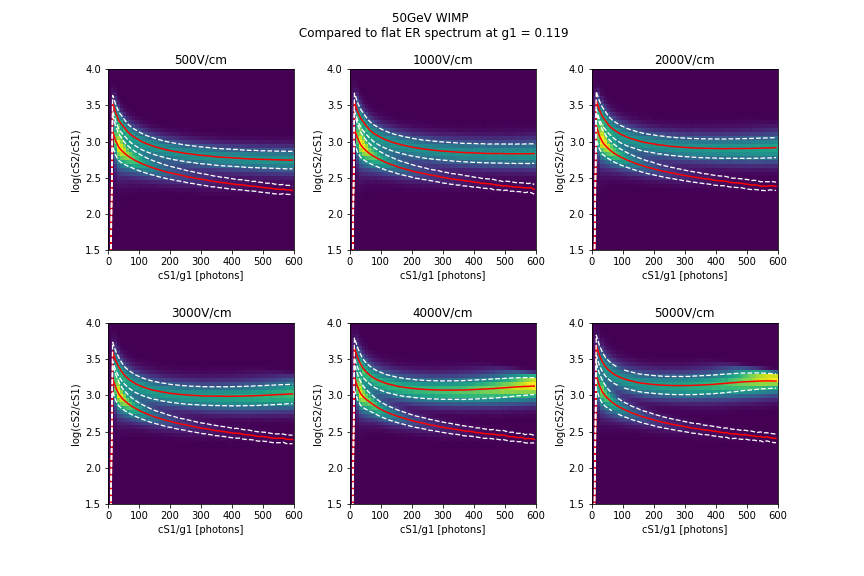
\includegraphics[width=0.99\columnwidth,clip,trim=70 40 70 50]{fig_wimperhistos.png}
\caption{Histograms for a flat electronic recoil spectrum and a nuclear recoil spectrum as from a 50~GeV spin-independent WIMP, simulated for different electric fields. The top band for each plot is the electronic recoil band, the bottom is the nuclear recoil band. Red lines refer to the median for either band, and the white dotted lines are the one-sigma region.}\label{fig:wimperhistos}
\end{center}
\end{figure}

The results of simulating events from a type of source, be it electronic or nuclear recoils, are a list of S1 and S2 values for each event. Binning these events into a 2D~histogram will show how a given type of interaction looks like in terms of the signals received. An example shown in \autoref{fig:wimperhistos} is the histogram of a 50~GeV spin-independent WIMP, which is lower in S2 than that of electronic recoil events. This difference allows for distinction between these two types of interactions and can be measured quantitatively in a few ways. Leakage is the proportion of electronic recoil events per bin that lie below the nuclear recoil median line; rejection is the percentage of background events that are not in the region of interest given by $(1-\mathrm{leakage})$. Various instrumental parameters affect the discrimination capability. For example, the drift field affects the gap between the nuclear and electronic recoil spectra, as does the $g1$~parameter which measures the S1 light yield in the detector. As can be seen from \autoref{fig:wimperhistos}, even moderate drift fields provide satisfactory discrimination. Discrimination is also affected by the atomic structure of xenon, leading to increased leakage from neutrino and Compton scatters on L-shell electrons due to the accompanying atomic de-excitation via Auger electron cascades. This effect is still under study, but available measurements indicate a reduction in rejection by a factor of $6\times$ near the L-shell binding energy ($5.2\1{keV}$) compared to predictions from valence electronic recoils and $\beta$-decays~\cite{Temples:2019taup, Temples:2021prd}. Including this effect for the solar neutrino ER background results in an 8\% relative increase in leakage from 5.2--8 keV, for 50\% NR acceptance.

Importantly, already with the performance of running detectors, discrimination between electronic and nuclear recoils in liquid xenon is sufficient to achieve the various science goals presented in this review, whether they pertain to WIMPs, neutrino-induced signals in both the electronic and nuclear recoil band, or the search for neutrinoless double-beta decay. The accuracy of these simulation results is confirmed \textit{in situ} using dedicated calibration sources, such as dissolved gamma line sources ${}^{83\mathrm{m}}$Kr~\cite{Kastens:2009pa}, dissolved beta-spectrum sources ${}^{220}$Rn~\cite{Lang:2016zde,Aprile:2016pmc}, TH$_3$C~\cite{Akerib:2015wdi}, as well as various neutron sources~\cite{Collar:2013xva,Aprile:2013teh,Akerib:2016mzi}.

